%%
%% Completed: 2022/01/14
%% Copyright: Andy GAO (华工自动化)
%%
%%==========================================================
%%          华南理工大学博士学位论文——扉页
%%      Author: Andy GAO        Date: 2022.01.
%%==========================================================
%%
\clearpage
\pagestyle{empty}


%%==========================================================
%% 封面
%%==========================================================
\begin{center}
%
\noindent

\vspace{2.5cm}

%
%%%%%%%%%%%%%%%%%%%%%%%%%%%%%%%%%%%%%%%%%%%%%%%%%%%%% Figure
\begin{figure}[!h]
  \centering
  
\includegraphics[width=12.1cm,height=2.76cm]{TITLEPAGE/FIGs/SCUTemblem} % 校徽
  %\caption{}
  %\label{fig:}
\end{figure}
%%%%%%%%%%%%%%%%%%%%%%%%%%%%%%%%%%%%%%%%%%%%%%%%%%%%% End Figure
%

\vspace{0.5em}
{\heiti\chuhao
\makebox[9.1cm][s]{课程设计报告}
}\\

\vspace{2.5cm}

{\heiti\erhao
% 若题目太长，则手动截断（此处放置第一段）
\uline{\hfill{UR5e 机械臂视觉伺服课程设计报告}\hfill}\\
% 若题目太长，则手动截断（此处放置第二段）
% \uline{\hfill{LaTeX模板介绍与案例说明}\hfill}\\
}

\vspace{3cm}


\ifSingleBlindReview
%%----------------------------------------------------------
%% 单盲评审/终版提交封面
%%----------------------------------------------------------

\begin{minipage}[!h]{0.75\linewidth}
\centering
\heiti\sanhao
\makebox[4cm][s]{作者姓名}~~\uline{\hfill{张杰钧}\hfill}\\
\makebox[4cm][s]{学科专业}~~\uline{\hfill{机械}\hfill}\\
\makebox[4cm][s]{指导教师}~~\uline{\hfill{徐大波{\quad}教~授}\hfill}\\
\makebox[4cm][s]{所在学院}~~\uline{\hfill{吴贤铭智能工程学院}\hfill}\\
\makebox[4cm][s]{论文提交日期}~~\uline{\hfill{\thesissubmitdate}\hfill}\\
\end{minipage}



\else
%%----------------------------------------------------------
%% 双盲评审封面
%%----------------------------------------------------------

\begin{minipage}[!h]{0.75\linewidth}
\centering
\heiti\sanhao
\makebox[4cm][s]{学科专业}~~\uline{\hfill{控制科学与工程}\hfill}\\
\makebox[4cm][s]{所在学院}~~\uline{\hfill{吴贤铭智能工程学院}\hfill}\\
\makebox[4cm][s]{论文提交日期}~~\uline{\hfill{\thesissubmitdate}\hfill}\\
\end{minipage}

\vfill

% 论文评审结果处理办法
\newpage
\null
\noindent
\centering

\vspace{3cm}

%
%%%%%%%%%%%%%%%%%%%%%%%%%%%%%%%%%%%%%%%%%%%%%%%%%%%%% Figure
\begin{figure}[!h]
  \centering
  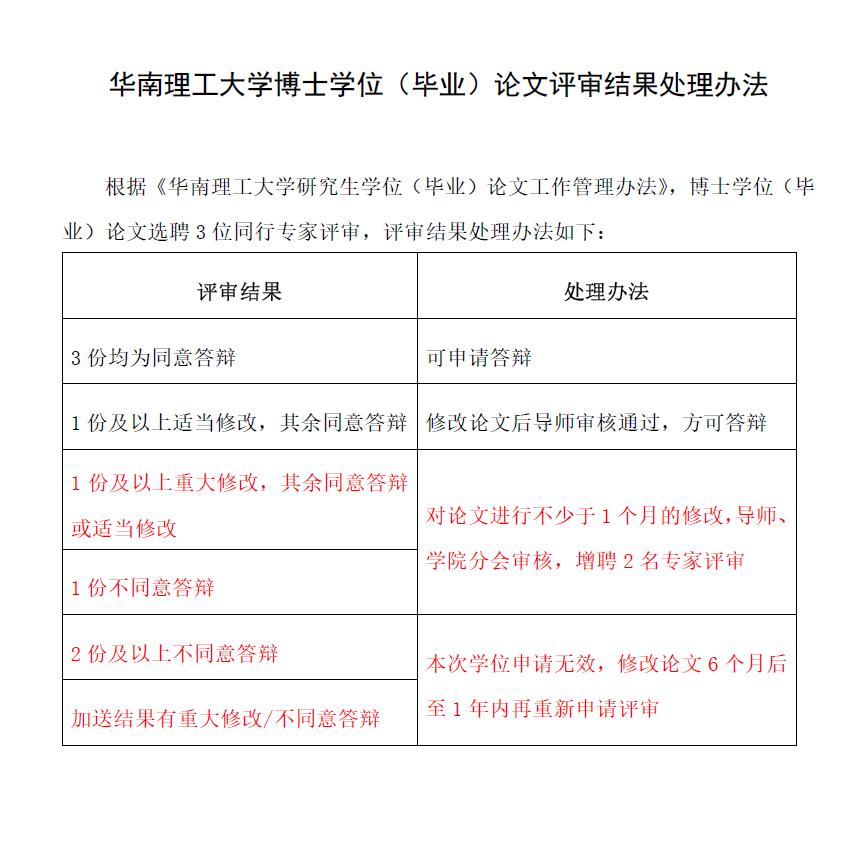
\includegraphics[width=\linewidth]{TITLEPAGE/FIGs/PingShenChuLi} % 评审结果处理办法
  %\caption{}
  %\label{fig:}
\end{figure}
%%%%%%%%%%%%%%%%%%%%%%%%%%%%%%%%%%%%%%%%%%%%%%%%%%%%% End Figure
%


\fi
%
\end{center}

\vfill





\ifSingleBlindReview
%%----------------------------------------------------------
%% 单盲评审/终版提交内封、题名页、授权书
%%----------------------------------------------------------
%%==========================================================
%% 英文内封
%%==========================================================
\newpage
\begin{center}
%
\noindent

\vspace{4cm}

%% 论文的英文标题
\textbf{{\xiaoerhao
IBVS Control of UR5e Manipulator
}}

\vspace{2cm}

{\sihao
A Report Submitted for the Course of \textit{Fundamentals of Control for Embodied Intelligent Systems}
}

\vspace{3cm}

\begin{minipage}[!h]{0.4\linewidth}
\raggedright        % 左对齐
\textbf{\xiaosanhao
\makebox[2.8cm][s]{Candidate:}  Zhang~Jiejun \hfill\\
\makebox[2.8cm][s]{Supervisor:}  Prof. Xu~Dabo \hfill\\
}
\end{minipage}

\vspace{3.5cm}

{\xiaosanhao
South China University of Technology \par
Guangzhou, China
}

%
\end{center}

\vfill

\baselineskip=1\baselineskip    % 调整行距
\normalsize                     % 后文字体：小四宋体


%%
%% Copyright: Andy GAO (华工自动化)
%%
%%==========================================================
%%          华南理工大学博士学位论文——扉页
%%      Author: Andy GAO        Date: 2022.01.
%%==========================================================
%%